
%(BEGIN_QUESTION)
% Copyright 2012, Tony R. Kuphaldt, released under the Creative Commons Attribution License (v 1.0)
% This means you may do almost anything with this work of mine, so long as you give me proper credit

A triple-redundant temperature control system is implemented using FOUNDATION Fieldbus technology.  A general P\&ID of the control scheme is shown here, followed by the Fieldbus function block diagram:

$$\includegraphics[width=15.5cm]{i02133x02.eps}$$

$$\includegraphics[width=15.5cm]{i02133x01.eps}$$

The ISEL function block selects the median signal from the three temperature transmitters, and is able to operate even if only one of those temperature signals is good.

\filbreak

Calculate the probability of system failure given the following device failure probabilites:

\begin{itemize}
\item{} TT-101a = 0.001
\item{} TT-101b = 0.001
\item{} TT-101c = 0.001
\item{} TV-101 = 0.003
\end{itemize}

\vskip 10pt

Now, suppose the ISEL function block were moved from TT-101a to TV-101.  Re-calculate the probability of system failure given the same device failure probabilities.

\underbar{file i02133}
%(END_QUESTION)





%(BEGIN_ANSWER)

Probability of system failure with ISEL block located in TT-101a = 0.003997001

$$\includegraphics[width=15.5cm]{i02133x03.eps}$$

\vskip 20pt

Probability of system failure with ISEL block located in TV-101 = 0.003000001

$$\includegraphics[width=15.5cm]{i02133x04.eps}$$

%(END_ANSWER)





%(BEGIN_NOTES)



%(END_NOTES)


